% Options for packages loaded elsewhere
\PassOptionsToPackage{unicode}{hyperref}
\PassOptionsToPackage{hyphens}{url}
\PassOptionsToPackage{dvipsnames,svgnames,x11names}{xcolor}
%
\documentclass[
  letterpaper,
  DIV=11,
  numbers=noendperiod]{scrartcl}

\usepackage{amsmath,amssymb}
\usepackage{iftex}
\ifPDFTeX
  \usepackage[T1]{fontenc}
  \usepackage[utf8]{inputenc}
  \usepackage{textcomp} % provide euro and other symbols
\else % if luatex or xetex
  \usepackage{unicode-math}
  \defaultfontfeatures{Scale=MatchLowercase}
  \defaultfontfeatures[\rmfamily]{Ligatures=TeX,Scale=1}
\fi
\usepackage{lmodern}
\ifPDFTeX\else  
    % xetex/luatex font selection
\fi
% Use upquote if available, for straight quotes in verbatim environments
\IfFileExists{upquote.sty}{\usepackage{upquote}}{}
\IfFileExists{microtype.sty}{% use microtype if available
  \usepackage[]{microtype}
  \UseMicrotypeSet[protrusion]{basicmath} % disable protrusion for tt fonts
}{}
\makeatletter
\@ifundefined{KOMAClassName}{% if non-KOMA class
  \IfFileExists{parskip.sty}{%
    \usepackage{parskip}
  }{% else
    \setlength{\parindent}{0pt}
    \setlength{\parskip}{6pt plus 2pt minus 1pt}}
}{% if KOMA class
  \KOMAoptions{parskip=half}}
\makeatother
\usepackage{xcolor}
\setlength{\emergencystretch}{3em} % prevent overfull lines
\setcounter{secnumdepth}{-\maxdimen} % remove section numbering
% Make \paragraph and \subparagraph free-standing
\ifx\paragraph\undefined\else
  \let\oldparagraph\paragraph
  \renewcommand{\paragraph}[1]{\oldparagraph{#1}\mbox{}}
\fi
\ifx\subparagraph\undefined\else
  \let\oldsubparagraph\subparagraph
  \renewcommand{\subparagraph}[1]{\oldsubparagraph{#1}\mbox{}}
\fi

\usepackage{color}
\usepackage{fancyvrb}
\newcommand{\VerbBar}{|}
\newcommand{\VERB}{\Verb[commandchars=\\\{\}]}
\DefineVerbatimEnvironment{Highlighting}{Verbatim}{commandchars=\\\{\}}
% Add ',fontsize=\small' for more characters per line
\usepackage{framed}
\definecolor{shadecolor}{RGB}{241,243,245}
\newenvironment{Shaded}{\begin{snugshade}}{\end{snugshade}}
\newcommand{\AlertTok}[1]{\textcolor[rgb]{0.68,0.00,0.00}{#1}}
\newcommand{\AnnotationTok}[1]{\textcolor[rgb]{0.37,0.37,0.37}{#1}}
\newcommand{\AttributeTok}[1]{\textcolor[rgb]{0.40,0.45,0.13}{#1}}
\newcommand{\BaseNTok}[1]{\textcolor[rgb]{0.68,0.00,0.00}{#1}}
\newcommand{\BuiltInTok}[1]{\textcolor[rgb]{0.00,0.23,0.31}{#1}}
\newcommand{\CharTok}[1]{\textcolor[rgb]{0.13,0.47,0.30}{#1}}
\newcommand{\CommentTok}[1]{\textcolor[rgb]{0.37,0.37,0.37}{#1}}
\newcommand{\CommentVarTok}[1]{\textcolor[rgb]{0.37,0.37,0.37}{\textit{#1}}}
\newcommand{\ConstantTok}[1]{\textcolor[rgb]{0.56,0.35,0.01}{#1}}
\newcommand{\ControlFlowTok}[1]{\textcolor[rgb]{0.00,0.23,0.31}{#1}}
\newcommand{\DataTypeTok}[1]{\textcolor[rgb]{0.68,0.00,0.00}{#1}}
\newcommand{\DecValTok}[1]{\textcolor[rgb]{0.68,0.00,0.00}{#1}}
\newcommand{\DocumentationTok}[1]{\textcolor[rgb]{0.37,0.37,0.37}{\textit{#1}}}
\newcommand{\ErrorTok}[1]{\textcolor[rgb]{0.68,0.00,0.00}{#1}}
\newcommand{\ExtensionTok}[1]{\textcolor[rgb]{0.00,0.23,0.31}{#1}}
\newcommand{\FloatTok}[1]{\textcolor[rgb]{0.68,0.00,0.00}{#1}}
\newcommand{\FunctionTok}[1]{\textcolor[rgb]{0.28,0.35,0.67}{#1}}
\newcommand{\ImportTok}[1]{\textcolor[rgb]{0.00,0.46,0.62}{#1}}
\newcommand{\InformationTok}[1]{\textcolor[rgb]{0.37,0.37,0.37}{#1}}
\newcommand{\KeywordTok}[1]{\textcolor[rgb]{0.00,0.23,0.31}{#1}}
\newcommand{\NormalTok}[1]{\textcolor[rgb]{0.00,0.23,0.31}{#1}}
\newcommand{\OperatorTok}[1]{\textcolor[rgb]{0.37,0.37,0.37}{#1}}
\newcommand{\OtherTok}[1]{\textcolor[rgb]{0.00,0.23,0.31}{#1}}
\newcommand{\PreprocessorTok}[1]{\textcolor[rgb]{0.68,0.00,0.00}{#1}}
\newcommand{\RegionMarkerTok}[1]{\textcolor[rgb]{0.00,0.23,0.31}{#1}}
\newcommand{\SpecialCharTok}[1]{\textcolor[rgb]{0.37,0.37,0.37}{#1}}
\newcommand{\SpecialStringTok}[1]{\textcolor[rgb]{0.13,0.47,0.30}{#1}}
\newcommand{\StringTok}[1]{\textcolor[rgb]{0.13,0.47,0.30}{#1}}
\newcommand{\VariableTok}[1]{\textcolor[rgb]{0.07,0.07,0.07}{#1}}
\newcommand{\VerbatimStringTok}[1]{\textcolor[rgb]{0.13,0.47,0.30}{#1}}
\newcommand{\WarningTok}[1]{\textcolor[rgb]{0.37,0.37,0.37}{\textit{#1}}}

\providecommand{\tightlist}{%
  \setlength{\itemsep}{0pt}\setlength{\parskip}{0pt}}\usepackage{longtable,booktabs,array}
\usepackage{calc} % for calculating minipage widths
% Correct order of tables after \paragraph or \subparagraph
\usepackage{etoolbox}
\makeatletter
\patchcmd\longtable{\par}{\if@noskipsec\mbox{}\fi\par}{}{}
\makeatother
% Allow footnotes in longtable head/foot
\IfFileExists{footnotehyper.sty}{\usepackage{footnotehyper}}{\usepackage{footnote}}
\makesavenoteenv{longtable}
\usepackage{graphicx}
\makeatletter
\def\maxwidth{\ifdim\Gin@nat@width>\linewidth\linewidth\else\Gin@nat@width\fi}
\def\maxheight{\ifdim\Gin@nat@height>\textheight\textheight\else\Gin@nat@height\fi}
\makeatother
% Scale images if necessary, so that they will not overflow the page
% margins by default, and it is still possible to overwrite the defaults
% using explicit options in \includegraphics[width, height, ...]{}
\setkeys{Gin}{width=\maxwidth,height=\maxheight,keepaspectratio}
% Set default figure placement to htbp
\makeatletter
\def\fps@figure{htbp}
\makeatother

\KOMAoption{captions}{tableheading}
\makeatletter
\makeatother
\makeatletter
\makeatother
\makeatletter
\@ifpackageloaded{caption}{}{\usepackage{caption}}
\AtBeginDocument{%
\ifdefined\contentsname
  \renewcommand*\contentsname{Table of contents}
\else
  \newcommand\contentsname{Table of contents}
\fi
\ifdefined\listfigurename
  \renewcommand*\listfigurename{List of Figures}
\else
  \newcommand\listfigurename{List of Figures}
\fi
\ifdefined\listtablename
  \renewcommand*\listtablename{List of Tables}
\else
  \newcommand\listtablename{List of Tables}
\fi
\ifdefined\figurename
  \renewcommand*\figurename{Figure}
\else
  \newcommand\figurename{Figure}
\fi
\ifdefined\tablename
  \renewcommand*\tablename{Table}
\else
  \newcommand\tablename{Table}
\fi
}
\@ifpackageloaded{float}{}{\usepackage{float}}
\floatstyle{ruled}
\@ifundefined{c@chapter}{\newfloat{codelisting}{h}{lop}}{\newfloat{codelisting}{h}{lop}[chapter]}
\floatname{codelisting}{Listing}
\newcommand*\listoflistings{\listof{codelisting}{List of Listings}}
\makeatother
\makeatletter
\@ifpackageloaded{caption}{}{\usepackage{caption}}
\@ifpackageloaded{subcaption}{}{\usepackage{subcaption}}
\makeatother
\makeatletter
\@ifpackageloaded{tcolorbox}{}{\usepackage[skins,breakable]{tcolorbox}}
\makeatother
\makeatletter
\@ifundefined{shadecolor}{\definecolor{shadecolor}{rgb}{.97, .97, .97}}
\makeatother
\makeatletter
\makeatother
\makeatletter
\makeatother
\ifLuaTeX
  \usepackage{selnolig}  % disable illegal ligatures
\fi
\IfFileExists{bookmark.sty}{\usepackage{bookmark}}{\usepackage{hyperref}}
\IfFileExists{xurl.sty}{\usepackage{xurl}}{} % add URL line breaks if available
\urlstyle{same} % disable monospaced font for URLs
\hypersetup{
  pdftitle={STL\_HEALTH\_Lead},
  colorlinks=true,
  linkcolor={blue},
  filecolor={Maroon},
  citecolor={Blue},
  urlcolor={Blue},
  pdfcreator={LaTeX via pandoc}}

\title{STL\_HEALTH\_Lead}
\author{}
\date{}

\begin{document}
\maketitle
\ifdefined\Shaded\renewenvironment{Shaded}{\begin{tcolorbox}[borderline west={3pt}{0pt}{shadecolor}, breakable, enhanced, sharp corners, frame hidden, interior hidden, boxrule=0pt]}{\end{tcolorbox}}\fi

\hypertarget{stl_health_lead}{%
\section{STL\_HEALTH\_Lead}\label{stl_health_lead}}

\emph{ABSTRACT from GitHub repository:} ``This repository contains a map
image of census tracts in St.~Louis, Missouri, colored by the estimated
number of high blood lead tests over the 2010-2015 period. The
repository also contains a variety of plots describing high lead
exposure in St.~Louis and two demographic correlates - race and
poverty.''

Here, we will conduct data exploration and visualization with the
stl\_blood\_lead.csv file.

\begin{Shaded}
\begin{Highlighting}[]
\FunctionTok{library}\NormalTok{(tidyverse)}
\end{Highlighting}
\end{Shaded}

\begin{verbatim}
-- Attaching core tidyverse packages ------------------------ tidyverse 2.0.0 --
v dplyr     1.1.4     v readr     2.1.5
v forcats   1.0.0     v stringr   1.5.1
v ggplot2   3.5.2     v tibble    3.3.0
v lubridate 1.9.4     v tidyr     1.3.1
v purrr     1.1.0     
-- Conflicts ------------------------------------------ tidyverse_conflicts() --
x dplyr::filter() masks stats::filter()
x dplyr::lag()    masks stats::lag()
i Use the conflicted package (<http://conflicted.r-lib.org/>) to force all conflicts to become errors
\end{verbatim}

\begin{Shaded}
\begin{Highlighting}[]
\FunctionTok{library}\NormalTok{(janitor)}
\end{Highlighting}
\end{Shaded}

\begin{verbatim}

Attaching package: 'janitor'

The following objects are masked from 'package:stats':

    chisq.test, fisher.test
\end{verbatim}

\begin{Shaded}
\begin{Highlighting}[]
\FunctionTok{library}\NormalTok{(here)}
\end{Highlighting}
\end{Shaded}

\begin{verbatim}
here() starts at /Users/vedikashirtekar/Documents/MEDS/EDS-212/eds-221-day1-activity-vedika
\end{verbatim}

\begin{Shaded}
\begin{Highlighting}[]
\NormalTok{stl\_lead }\OtherTok{\textless{}{-}} \FunctionTok{read.csv}\NormalTok{(here}\SpecialCharTok{::}\FunctionTok{here}\NormalTok{(}\StringTok{"data"}\NormalTok{, }\StringTok{"stl\_blood\_lead.csv"}\NormalTok{))}

\CommentTok{\# view summary of dataset}
\NormalTok{skimr}\SpecialCharTok{::}\FunctionTok{skim}\NormalTok{(stl\_lead)}
\end{Highlighting}
\end{Shaded}

\begin{longtable}[]{@{}ll@{}}
\caption{Data summary}\tabularnewline
\toprule\noalign{}
\endfirsthead
\endhead
\bottomrule\noalign{}
\endlastfoot
Name & stl\_lead \\
Number of rows & 106 \\
Number of columns & 15 \\
\_\_\_\_\_\_\_\_\_\_\_\_\_\_\_\_\_\_\_\_\_\_\_ & \\
Column type frequency: & \\
character & 1 \\
numeric & 14 \\
\_\_\_\_\_\_\_\_\_\_\_\_\_\_\_\_\_\_\_\_\_\_\_\_ & \\
Group variables & None \\
\end{longtable}

\textbf{Variable type: character}

\begin{longtable}[]{@{}
  >{\raggedright\arraybackslash}p{(\columnwidth - 14\tabcolsep) * \real{0.1944}}
  >{\raggedleft\arraybackslash}p{(\columnwidth - 14\tabcolsep) * \real{0.1389}}
  >{\raggedleft\arraybackslash}p{(\columnwidth - 14\tabcolsep) * \real{0.1944}}
  >{\raggedleft\arraybackslash}p{(\columnwidth - 14\tabcolsep) * \real{0.0556}}
  >{\raggedleft\arraybackslash}p{(\columnwidth - 14\tabcolsep) * \real{0.0556}}
  >{\raggedleft\arraybackslash}p{(\columnwidth - 14\tabcolsep) * \real{0.0833}}
  >{\raggedleft\arraybackslash}p{(\columnwidth - 14\tabcolsep) * \real{0.1250}}
  >{\raggedleft\arraybackslash}p{(\columnwidth - 14\tabcolsep) * \real{0.1528}}@{}}
\toprule\noalign{}
\begin{minipage}[b]{\linewidth}\raggedright
skim\_variable
\end{minipage} & \begin{minipage}[b]{\linewidth}\raggedleft
n\_missing
\end{minipage} & \begin{minipage}[b]{\linewidth}\raggedleft
complete\_rate
\end{minipage} & \begin{minipage}[b]{\linewidth}\raggedleft
min
\end{minipage} & \begin{minipage}[b]{\linewidth}\raggedleft
max
\end{minipage} & \begin{minipage}[b]{\linewidth}\raggedleft
empty
\end{minipage} & \begin{minipage}[b]{\linewidth}\raggedleft
n\_unique
\end{minipage} & \begin{minipage}[b]{\linewidth}\raggedleft
whitespace
\end{minipage} \\
\midrule\noalign{}
\endhead
\bottomrule\noalign{}
\endlastfoot
nameLSAD & 0 & 1 & 17 & 20 & 0 & 106 & 0 \\
\end{longtable}

\textbf{Variable type: numeric}

\begin{longtable}[]{@{}
  >{\raggedright\arraybackslash}p{(\columnwidth - 20\tabcolsep) * \real{0.1154}}
  >{\raggedleft\arraybackslash}p{(\columnwidth - 20\tabcolsep) * \real{0.0769}}
  >{\raggedleft\arraybackslash}p{(\columnwidth - 20\tabcolsep) * \real{0.1077}}
  >{\raggedleft\arraybackslash}p{(\columnwidth - 20\tabcolsep) * \real{0.1000}}
  >{\raggedleft\arraybackslash}p{(\columnwidth - 20\tabcolsep) * \real{0.0615}}
  >{\raggedleft\arraybackslash}p{(\columnwidth - 20\tabcolsep) * \real{0.0923}}
  >{\raggedleft\arraybackslash}p{(\columnwidth - 20\tabcolsep) * \real{0.1000}}
  >{\raggedleft\arraybackslash}p{(\columnwidth - 20\tabcolsep) * \real{0.1000}}
  >{\raggedleft\arraybackslash}p{(\columnwidth - 20\tabcolsep) * \real{0.1000}}
  >{\raggedleft\arraybackslash}p{(\columnwidth - 20\tabcolsep) * \real{0.1000}}
  >{\raggedright\arraybackslash}p{(\columnwidth - 20\tabcolsep) * \real{0.0462}}@{}}
\toprule\noalign{}
\begin{minipage}[b]{\linewidth}\raggedright
skim\_variable
\end{minipage} & \begin{minipage}[b]{\linewidth}\raggedleft
n\_missing
\end{minipage} & \begin{minipage}[b]{\linewidth}\raggedleft
complete\_rate
\end{minipage} & \begin{minipage}[b]{\linewidth}\raggedleft
mean
\end{minipage} & \begin{minipage}[b]{\linewidth}\raggedleft
sd
\end{minipage} & \begin{minipage}[b]{\linewidth}\raggedleft
p0
\end{minipage} & \begin{minipage}[b]{\linewidth}\raggedleft
p25
\end{minipage} & \begin{minipage}[b]{\linewidth}\raggedleft
p50
\end{minipage} & \begin{minipage}[b]{\linewidth}\raggedleft
p75
\end{minipage} & \begin{minipage}[b]{\linewidth}\raggedleft
p100
\end{minipage} & \begin{minipage}[b]{\linewidth}\raggedright
hist
\end{minipage} \\
\midrule\noalign{}
\endhead
\bottomrule\noalign{}
\endlastfoot
geoID & 0 & 1 & 2.951011e+10 & 8132.85 & 29510101100 & 2.951011e+10 &
2.951011e+10 & 2.951012e+10 & 2.951013e+10 & ▇▇▆▃▆ \\
tractCE & 0 & 1 & 1.133859e+05 & 8132.85 & 101100 & 1.064250e+05 &
1.123500e+05 & 1.191018e+05 & 1.276000e+05 & ▇▇▆▃▆ \\
countTested & 0 & 1 & 7.373700e+02 & 414.18 & 23 & 4.110000e+02 &
6.940000e+02 & 9.232500e+02 & 2.116000e+03 & ▆▇▅▂▁ \\
pctElevated & 0 & 1 & 1.016000e+01 & 6.01 & 0 & 4.590000e+00 &
9.480000e+00 & 1.438000e+01 & 2.328000e+01 & ▇▇▇▅▃ \\
totalPop & 0 & 1 & 2.998580e+03 & 1263.14 & 620 & 2.025000e+03 &
2.911500e+03 & 3.784500e+03 & 7.069000e+03 & ▅▇▆▂▁ \\
totalPop\_MOE & 0 & 1 & 3.533500e+02 & 140.30 & 94 & 2.495000e+02 &
3.335000e+02 & 4.395000e+02 & 8.320000e+02 & ▅▇▃▂▁ \\
white & 0 & 1 & 1.371720e+03 & 1293.40 & 1 & 8.850000e+01 & 1.290000e+03
& 2.168250e+03 & 6.128000e+03 & ▇▅▃▁▁ \\
white\_MOE & 0 & 1 & 2.013800e+02 & 145.21 & 4 & 6.050000e+01 &
2.125000e+02 & 2.997500e+02 & 7.510000e+02 & ▇▇▅▁▁ \\
black & 0 & 1 & 1.429870e+03 & 1038.31 & 35 & 6.332500e+02 &
1.334500e+03 & 2.029000e+03 & 4.572000e+03 & ▇▆▃▂▁ \\
black\_MOE & 0 & 1 & 2.883800e+02 & 148.84 & 38 & 1.832500e+02 &
2.690000e+02 & 3.792500e+02 & 7.600000e+02 & ▆▇▆▂▁ \\
povertyTot & 0 & 1 & 7.869400e+02 & 528.61 & 158 & 4.085000e+02 &
6.515000e+02 & 9.557500e+02 & 2.801000e+03 & ▇▅▂▁▁ \\
povertyTot\_MOE & 0 & 1 & 2.705000e+02 & 156.11 & 65 & 1.602500e+02 &
2.415000e+02 & 3.375000e+02 & 1.049000e+03 & ▇▅▁▁▁ \\
povertyU18 & 0 & 1 & 2.497500e+02 & 262.60 & 0 & 6.650000e+01 &
1.735000e+02 & 3.417500e+02 & 1.320000e+03 & ▇▂▁▁▁ \\
povertyU18\_MOE & 0 & 1 & 1.400800e+02 & 107.48 & 3 & 6.125000e+01 &
1.205000e+02 & 1.947500e+02 & 5.950000e+02 & ▇▆▂▁▁ \\
\end{longtable}

Now, we will look at some basic data visualization and cleaning on this
dataset using skimr and ggplot.

\begin{Shaded}
\begin{Highlighting}[]
\NormalTok{stl\_lead }\OtherTok{\textless{}{-}}\NormalTok{ stl\_lead }\SpecialCharTok{\%\textgreater{}\%} \FunctionTok{clean\_names}\NormalTok{()}
\FunctionTok{names}\NormalTok{(stl\_lead)}
\end{Highlighting}
\end{Shaded}

\begin{verbatim}
 [1] "geo_id"          "tract_ce"        "name_lsad"       "count_tested"   
 [5] "pct_elevated"    "total_pop"       "total_pop_moe"   "white"          
 [9] "white_moe"       "black"           "black_moe"       "poverty_tot"    
[13] "poverty_tot_moe" "poverty_u18"     "poverty_u18_moe"
\end{verbatim}

\begin{Shaded}
\begin{Highlighting}[]
\CommentTok{\# now that the column names are cleaned up, let\textquotesingle{}s visualize the distributions and summary of each column }
\NormalTok{skimr}\SpecialCharTok{::}\FunctionTok{skim}\NormalTok{(stl\_lead)}
\end{Highlighting}
\end{Shaded}

\begin{longtable}[]{@{}ll@{}}
\caption{Data summary}\tabularnewline
\toprule\noalign{}
\endfirsthead
\endhead
\bottomrule\noalign{}
\endlastfoot
Name & stl\_lead \\
Number of rows & 106 \\
Number of columns & 15 \\
\_\_\_\_\_\_\_\_\_\_\_\_\_\_\_\_\_\_\_\_\_\_\_ & \\
Column type frequency: & \\
character & 1 \\
numeric & 14 \\
\_\_\_\_\_\_\_\_\_\_\_\_\_\_\_\_\_\_\_\_\_\_\_\_ & \\
Group variables & None \\
\end{longtable}

\textbf{Variable type: character}

\begin{longtable}[]{@{}
  >{\raggedright\arraybackslash}p{(\columnwidth - 14\tabcolsep) * \real{0.1944}}
  >{\raggedleft\arraybackslash}p{(\columnwidth - 14\tabcolsep) * \real{0.1389}}
  >{\raggedleft\arraybackslash}p{(\columnwidth - 14\tabcolsep) * \real{0.1944}}
  >{\raggedleft\arraybackslash}p{(\columnwidth - 14\tabcolsep) * \real{0.0556}}
  >{\raggedleft\arraybackslash}p{(\columnwidth - 14\tabcolsep) * \real{0.0556}}
  >{\raggedleft\arraybackslash}p{(\columnwidth - 14\tabcolsep) * \real{0.0833}}
  >{\raggedleft\arraybackslash}p{(\columnwidth - 14\tabcolsep) * \real{0.1250}}
  >{\raggedleft\arraybackslash}p{(\columnwidth - 14\tabcolsep) * \real{0.1528}}@{}}
\toprule\noalign{}
\begin{minipage}[b]{\linewidth}\raggedright
skim\_variable
\end{minipage} & \begin{minipage}[b]{\linewidth}\raggedleft
n\_missing
\end{minipage} & \begin{minipage}[b]{\linewidth}\raggedleft
complete\_rate
\end{minipage} & \begin{minipage}[b]{\linewidth}\raggedleft
min
\end{minipage} & \begin{minipage}[b]{\linewidth}\raggedleft
max
\end{minipage} & \begin{minipage}[b]{\linewidth}\raggedleft
empty
\end{minipage} & \begin{minipage}[b]{\linewidth}\raggedleft
n\_unique
\end{minipage} & \begin{minipage}[b]{\linewidth}\raggedleft
whitespace
\end{minipage} \\
\midrule\noalign{}
\endhead
\bottomrule\noalign{}
\endlastfoot
name\_lsad & 0 & 1 & 17 & 20 & 0 & 106 & 0 \\
\end{longtable}

\textbf{Variable type: numeric}

\begin{longtable}[]{@{}
  >{\raggedright\arraybackslash}p{(\columnwidth - 20\tabcolsep) * \real{0.1221}}
  >{\raggedleft\arraybackslash}p{(\columnwidth - 20\tabcolsep) * \real{0.0763}}
  >{\raggedleft\arraybackslash}p{(\columnwidth - 20\tabcolsep) * \real{0.1069}}
  >{\raggedleft\arraybackslash}p{(\columnwidth - 20\tabcolsep) * \real{0.0992}}
  >{\raggedleft\arraybackslash}p{(\columnwidth - 20\tabcolsep) * \real{0.0611}}
  >{\raggedleft\arraybackslash}p{(\columnwidth - 20\tabcolsep) * \real{0.0916}}
  >{\raggedleft\arraybackslash}p{(\columnwidth - 20\tabcolsep) * \real{0.0992}}
  >{\raggedleft\arraybackslash}p{(\columnwidth - 20\tabcolsep) * \real{0.0992}}
  >{\raggedleft\arraybackslash}p{(\columnwidth - 20\tabcolsep) * \real{0.0992}}
  >{\raggedleft\arraybackslash}p{(\columnwidth - 20\tabcolsep) * \real{0.0992}}
  >{\raggedright\arraybackslash}p{(\columnwidth - 20\tabcolsep) * \real{0.0458}}@{}}
\toprule\noalign{}
\begin{minipage}[b]{\linewidth}\raggedright
skim\_variable
\end{minipage} & \begin{minipage}[b]{\linewidth}\raggedleft
n\_missing
\end{minipage} & \begin{minipage}[b]{\linewidth}\raggedleft
complete\_rate
\end{minipage} & \begin{minipage}[b]{\linewidth}\raggedleft
mean
\end{minipage} & \begin{minipage}[b]{\linewidth}\raggedleft
sd
\end{minipage} & \begin{minipage}[b]{\linewidth}\raggedleft
p0
\end{minipage} & \begin{minipage}[b]{\linewidth}\raggedleft
p25
\end{minipage} & \begin{minipage}[b]{\linewidth}\raggedleft
p50
\end{minipage} & \begin{minipage}[b]{\linewidth}\raggedleft
p75
\end{minipage} & \begin{minipage}[b]{\linewidth}\raggedleft
p100
\end{minipage} & \begin{minipage}[b]{\linewidth}\raggedright
hist
\end{minipage} \\
\midrule\noalign{}
\endhead
\bottomrule\noalign{}
\endlastfoot
geo\_id & 0 & 1 & 2.951011e+10 & 8132.85 & 29510101100 & 2.951011e+10 &
2.951011e+10 & 2.951012e+10 & 2.951013e+10 & ▇▇▆▃▆ \\
tract\_ce & 0 & 1 & 1.133859e+05 & 8132.85 & 101100 & 1.064250e+05 &
1.123500e+05 & 1.191018e+05 & 1.276000e+05 & ▇▇▆▃▆ \\
count\_tested & 0 & 1 & 7.373700e+02 & 414.18 & 23 & 4.110000e+02 &
6.940000e+02 & 9.232500e+02 & 2.116000e+03 & ▆▇▅▂▁ \\
pct\_elevated & 0 & 1 & 1.016000e+01 & 6.01 & 0 & 4.590000e+00 &
9.480000e+00 & 1.438000e+01 & 2.328000e+01 & ▇▇▇▅▃ \\
total\_pop & 0 & 1 & 2.998580e+03 & 1263.14 & 620 & 2.025000e+03 &
2.911500e+03 & 3.784500e+03 & 7.069000e+03 & ▅▇▆▂▁ \\
total\_pop\_moe & 0 & 1 & 3.533500e+02 & 140.30 & 94 & 2.495000e+02 &
3.335000e+02 & 4.395000e+02 & 8.320000e+02 & ▅▇▃▂▁ \\
white & 0 & 1 & 1.371720e+03 & 1293.40 & 1 & 8.850000e+01 & 1.290000e+03
& 2.168250e+03 & 6.128000e+03 & ▇▅▃▁▁ \\
white\_moe & 0 & 1 & 2.013800e+02 & 145.21 & 4 & 6.050000e+01 &
2.125000e+02 & 2.997500e+02 & 7.510000e+02 & ▇▇▅▁▁ \\
black & 0 & 1 & 1.429870e+03 & 1038.31 & 35 & 6.332500e+02 &
1.334500e+03 & 2.029000e+03 & 4.572000e+03 & ▇▆▃▂▁ \\
black\_moe & 0 & 1 & 2.883800e+02 & 148.84 & 38 & 1.832500e+02 &
2.690000e+02 & 3.792500e+02 & 7.600000e+02 & ▆▇▆▂▁ \\
poverty\_tot & 0 & 1 & 7.869400e+02 & 528.61 & 158 & 4.085000e+02 &
6.515000e+02 & 9.557500e+02 & 2.801000e+03 & ▇▅▂▁▁ \\
poverty\_tot\_moe & 0 & 1 & 2.705000e+02 & 156.11 & 65 & 1.602500e+02 &
2.415000e+02 & 3.375000e+02 & 1.049000e+03 & ▇▅▁▁▁ \\
poverty\_u18 & 0 & 1 & 2.497500e+02 & 262.60 & 0 & 6.650000e+01 &
1.735000e+02 & 3.417500e+02 & 1.320000e+03 & ▇▂▁▁▁ \\
poverty\_u18\_moe & 0 & 1 & 1.400800e+02 & 107.48 & 3 & 6.125000e+01 &
1.205000e+02 & 1.947500e+02 & 5.950000e+02 & ▇▆▂▁▁ \\
\end{longtable}

\begin{Shaded}
\begin{Highlighting}[]
\CommentTok{\# now, add a column called prop\_white that returns the percent of each census tract identifying as white (variable white in the dataset divided by variable totalPop, times 100)}
\NormalTok{stl\_blood\_lead }\OtherTok{\textless{}{-}}\NormalTok{ stl\_lead }\SpecialCharTok{\%\textgreater{}\%} \FunctionTok{mutate}\NormalTok{(}\AttributeTok{prop\_white =}\NormalTok{ (white}\SpecialCharTok{/}\NormalTok{total\_pop)}\SpecialCharTok{*}\DecValTok{100}\NormalTok{)}
\FunctionTok{str}\NormalTok{(stl\_blood\_lead)}
\end{Highlighting}
\end{Shaded}

\begin{verbatim}
'data.frame':   106 obs. of  16 variables:
 $ geo_id         : num  2.95e+10 2.95e+10 2.95e+10 2.95e+10 2.95e+10 ...
 $ tract_ce       : int  118100 117400 126700 119102 126800 126900 108100 127000 127400 103700 ...
 $ name_lsad      : chr  "Census Tract 1181" "Census Tract 1174" "Census Tract 1267" "Census Tract 1191.02" ...
 $ count_tested   : int  345 871 458 182 486 1296 903 585 2116 417 ...
 $ pct_elevated   : num  9.57 12.06 18.12 2.2 4.73 ...
 $ total_pop      : int  1161 4307 1089 3237 3490 4590 3144 2052 5486 2408 ...
 $ total_pop_moe  : int  192 447 199 309 231 826 464 273 516 274 ...
 $ white          : int  414 2604 432 2008 3026 148 108 304 1777 2149 ...
 $ white_moe      : int  100 303 116 262 270 217 111 82 391 212 ...
 $ black          : int  724 1338 631 646 194 4320 3020 1739 3603 156 ...
 $ black_moe      : int  179 374 187 210 98 760 442 283 621 190 ...
 $ poverty_tot    : int  324 615 506 958 349 1743 652 331 2524 254 ...
 $ poverty_tot_moe: int  140 255 164 234 129 825 305 156 598 88 ...
 $ poverty_u18    : int  109 169 98 15 35 627 256 47 1110 15 ...
 $ poverty_u18_moe: int  105 156 60 25 47 595 136 79 318 23 ...
 $ prop_white     : num  35.7 60.5 39.7 62 86.7 ...
\end{verbatim}

Now, we will use our new dataset stl\_blood\_lead to explore how
demographics and elevated blood lead levels are related via a
scatterplot and histogram.

\begin{Shaded}
\begin{Highlighting}[]
\CommentTok{\# scatterplot}
\NormalTok{stl\_blood\_lead }\SpecialCharTok{\%\textgreater{}\%} \FunctionTok{ggplot}\NormalTok{(}\FunctionTok{aes}\NormalTok{(}\AttributeTok{x =}\NormalTok{ pct\_elevated, }\AttributeTok{y =}\NormalTok{ prop\_white, }\AttributeTok{col =}\NormalTok{ pct\_elevated)) }\SpecialCharTok{+} \FunctionTok{geom\_point}\NormalTok{() }\SpecialCharTok{+} \FunctionTok{theme\_bw}\NormalTok{() }\SpecialCharTok{+} \FunctionTok{labs}\NormalTok{(}\AttributeTok{title =} \StringTok{"Proportion of White Residents in Census Tracts Impacted by Elevated Blood Lead Levels"}\NormalTok{, }\AttributeTok{x =} \StringTok{"Elevated Blood Lead Level"}\NormalTok{, }\AttributeTok{y =} \StringTok{"Proportion of White Residents"}\NormalTok{, }\AttributeTok{caption =} \StringTok{"*Color scaled by elevated blood lead level"}\NormalTok{) }\SpecialCharTok{+} \FunctionTok{guides}\NormalTok{(}\AttributeTok{color =}\NormalTok{ F)}
\end{Highlighting}
\end{Shaded}

\begin{verbatim}
Warning: The `<scale>` argument of `guides()` cannot be `FALSE`. Use "none" instead as
of ggplot2 3.3.4.
\end{verbatim}

\begin{figure}[H]

{\centering 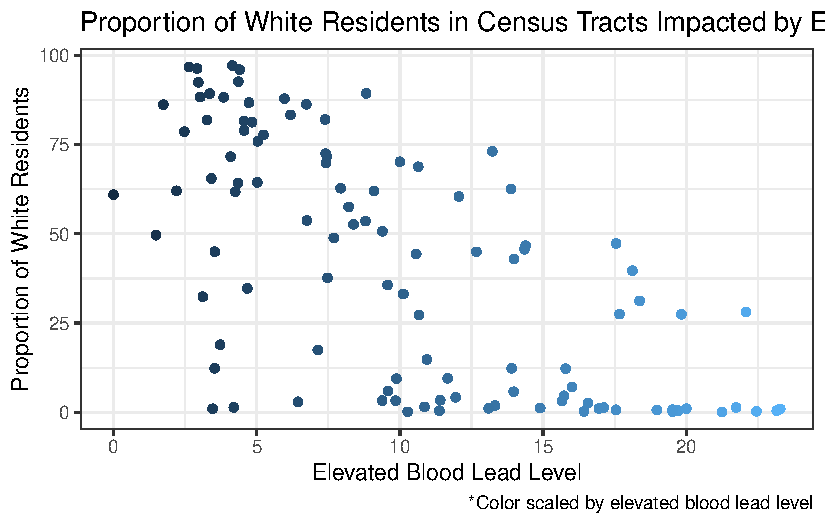
\includegraphics{stl_lead_inequity_files/figure-pdf/unnamed-chunk-3-1.pdf}

}

\end{figure}

\begin{Shaded}
\begin{Highlighting}[]
\FunctionTok{ggsave}\NormalTok{(here}\SpecialCharTok{::}\FunctionTok{here}\NormalTok{(}\StringTok{"figs"}\NormalTok{, }\StringTok{"stl\_scatter.png"}\NormalTok{))}
\end{Highlighting}
\end{Shaded}

\begin{verbatim}
Saving 5.5 x 3.5 in image
\end{verbatim}

\textbf{The trend indicates a decrease in the proportion of white
residents with higher blood lead levels. A higher proportion of white
residents in measured census tracts have lower elevated blood lead
levels compared to higher elevated blood lead levels. It is possible
that fewer white residents are impacted by lead pollution compared to
other demographics; however, this claim should be further investigated
for accuracy.}

\begin{Shaded}
\begin{Highlighting}[]
\NormalTok{stl\_blood\_lead }\SpecialCharTok{\%\textgreater{}\%} \FunctionTok{ggplot}\NormalTok{(}\FunctionTok{aes}\NormalTok{(}\AttributeTok{x =}\NormalTok{ pct\_elevated)) }\SpecialCharTok{+} \FunctionTok{geom\_histogram}\NormalTok{(}\AttributeTok{col =} \StringTok{"black"}\NormalTok{, }\AttributeTok{fill =} \StringTok{"darkblue"}\NormalTok{) }\SpecialCharTok{+} \FunctionTok{theme\_bw}\NormalTok{() }\SpecialCharTok{+}  \FunctionTok{labs}\NormalTok{(}\AttributeTok{title =} \StringTok{"Elevated Blood Lead Levels"}\NormalTok{, }\AttributeTok{x =} \StringTok{"Elevated Blood Lead Level"}\NormalTok{) }
\end{Highlighting}
\end{Shaded}

\begin{verbatim}
`stat_bin()` using `bins = 30`. Pick better value with `binwidth`.
\end{verbatim}

\begin{figure}[H]

{\centering 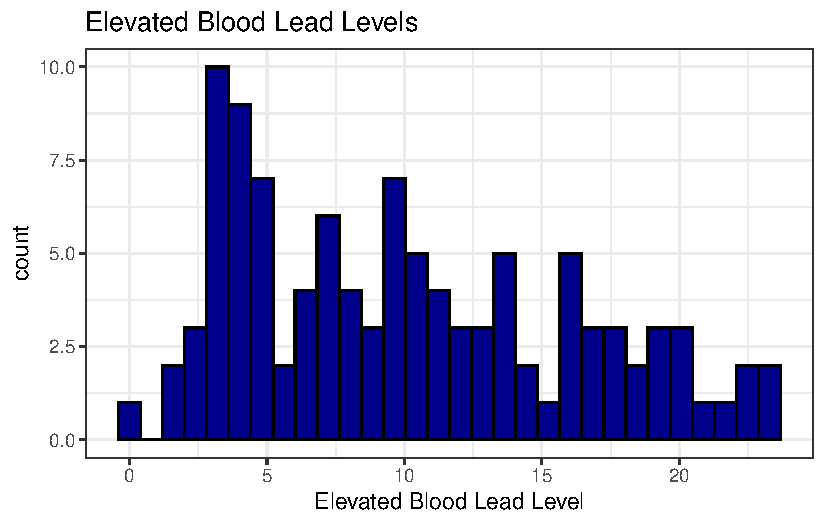
\includegraphics{stl_lead_inequity_files/figure-pdf/unnamed-chunk-4-1.pdf}

}

\end{figure}

\begin{Shaded}
\begin{Highlighting}[]
\FunctionTok{ggsave}\NormalTok{(here}\SpecialCharTok{::}\FunctionTok{here}\NormalTok{(}\StringTok{"figs"}\NormalTok{, }\StringTok{"stl\_hist.jpg"}\NormalTok{))}
\end{Highlighting}
\end{Shaded}

\begin{verbatim}
Saving 5.5 x 3.5 in image
`stat_bin()` using `bins = 30`. Pick better value with `binwidth`.
\end{verbatim}



\end{document}
